\documentclass[11pt,letterpaper]{article}

\usepackage{threeparttable}
\usepackage{textcomp,marvosym}
\usepackage{amsmath,amssymb}
\usepackage[left]{lineno}
\usepackage{changepage}
\usepackage{rotating}
\usepackage{natbib}
\usepackage{setspace}
\usepackage{fancyhdr}
\usepackage{graphicx}
\usepackage{booktabs}
\usepackage{pdfpages}
\usepackage{url}
\usepackage{longtable}
\usepackage{pdflscape}
\usepackage[outercaption]{sidecap}
\doublespacing

\raggedright
\textwidth = 6.5 in
\textheight = 9 in
\oddsidemargin = 0.0 in
\evensidemargin = 0.0 in
\topmargin = 0.0 in
\headheight = 0.0 in
\headsep = 0.0 in
\parskip = 0.1 in
\parindent = 0.2 in

\usepackage[aboveskip=1pt,labelfont=bf,labelsep=period,justification=raggedright,singlelinecheck=off]{caption}

%commands that were used to generate a PDF that was copied to make the .docx version for GSAB
%\pagestyle{empty}
%\usepackage[nomarkers,figuresonly]{endfloat}

\begin{document}

\begin{flushleft}
{\Large \textbf{The Precambrian paleogeography of Laurentia}}
\\

Nicholas L. Swanson-Hysell\textsuperscript{1}

\bigskip

\textsuperscript{1} Department of Earth and Planetary Science, University of California, Berkeley, CA 94720 USA

\end{flushleft}

\noindent\textit{This chapter is in preparation for the book Ancient Supercontinents and the Paleogeography of the Earth}

%\linenumbers

\section*{INTRODUCTION}

Laurentia was a major continent throughout the majority of the Proterozoic and is hypothesized to have been a central constituent of both the Paleoproterozoic Nuna and Neoproterozoic Rodinia supercontinents. The paleogeographic position of Laurentia is key to the development of reconstructions of Proterozoic paleogeography. There is a rich record of Precambrian paleomagnetic poles from Laurentia as well as an extensive geologic history of tectonism that are both key to evaluating and developing paleogeographic models.

\section*{Broad tectonic history overview}

Laurentia refers to the craton that forms the Precambrian core of North America (Fig. \ref{fig:Laurentia_map}). Laurentia is comprised of multiple Archean provinces that had unique histories prior to their amalgamation in the Paleoproterozoic, as well as tectonic zones of crustal growth that post-date this assembly \citep{Hoffman1989a, Whitmeyer2007a}. Collision between the Superior province and the composite Slave+Rae+Hearne+Nain provinces that resulted in the Trans-Hudson orogeny represents a major event in the formation of Laurentia \citep{Corrigan2009a}. Terminal collision recorded in the Trans-Hudson orogen is estimated to have been ca. 1.86 to 1.82 Ga based on constraints such as U-Pb dating of monazite grains and zircon rims \citep[e.g.]{Skipton2016a, Weller2017a}. A period of accretionary and collision orogenesis is recorded in the constituent provinces and terranes of Laurentia leading up to the terminal collision of the Trans-Hudson orogeny. This overall story of rapid Paleoproterozoic amalgamation of Laurentia's constituent Archean provinces, including the terminal Trans-Hudson orogeny, was synthesized in the seminal \textit{United Plates of America} paper of \citet{Hoffman1988a} and has been refined in the time since -- particularly with additional geochronological constraints. Of most relevance here are the events that led to the suturing of more major Archean provinces: the Thelon orogen associated with the collision between the Slave province and the Rae province ca. 2.0 to 1.9 Ga \citep{Hoffman1989a}; the Snowbird orogen associated with ca. 1.89 Ga collision between the Rae and Hearne provinces and associated terranes \citep{Berman2007a}; the Nagssugtoqidian orogen due to the ca. 1.86 to 1.84 Ga collision between the Rae and Nain provinces \citep{St-Onge2009a}; and the Torngat orogen resulting from the ca. 1.87 to 1.85 Ga collision of the Meta Incognita province (grouped with the Rae province in older compilations) with the Nain province \citep{St-Onge2009a}. As for the Wyoming province, many models posit that it was conjoined with Hearne and associated provinces as the time of the Trans-Hudson orogeny \citep[e.g.][]{St-Onge2009a, Pehrsson2015a} or was proximal to Hearne and Superior while still undergoing continued translation up to ca. 1.80 Ga \citep{Whitmeyer2007a}. A contrasting view has been been proposed that the Wyoming province and Medicine Hat blocks was not conjoined with the other Laurentia provinces until ca. 1.72 Ga \citep{Kilian2016a}. This interpretation is argued to be consistent with geochronological constraints on monazite and metamorphic zircon indicating active collisional orogenesis associated with the Big Sky orogen on the northern margin of the craton as late as ca. 1.75 to 1.72 Ga \citep{Condit2015a} and ca. 1.72 tectonomagmatic activity in the Black Hills region \citep{Redden1990a}. However, the evidence for earlier orogenesis ca. 1.78 to 1.75 in the Black Hills \citep{Dahl1999a,Hrncir2017a}, as well as high-grade tectonism as early as ca. 1.81 Ga in the Big Sky orogen \citep{Condit2015a}, may support the interpretation of \citet{Hrncir2017a} that ca. 1.72 Ga activity is a minor overprint on ca. 1.75 terminal suturing between Wyoming and Superior. Regardless, in both of these interpretations, Wyoming is a later addition to Laurentia with final suturing post-dating ca. 1.82 Ga amalgamation of Archean provinces with the Trans-Hudson orogen further to the northeast. Overall, the collision of these Archean microcontinents between ca. 1.9 and 1.8 Ga lead to rapid amalgamation of the majority of the Laurentia craton.

\begin{figure}
\centering
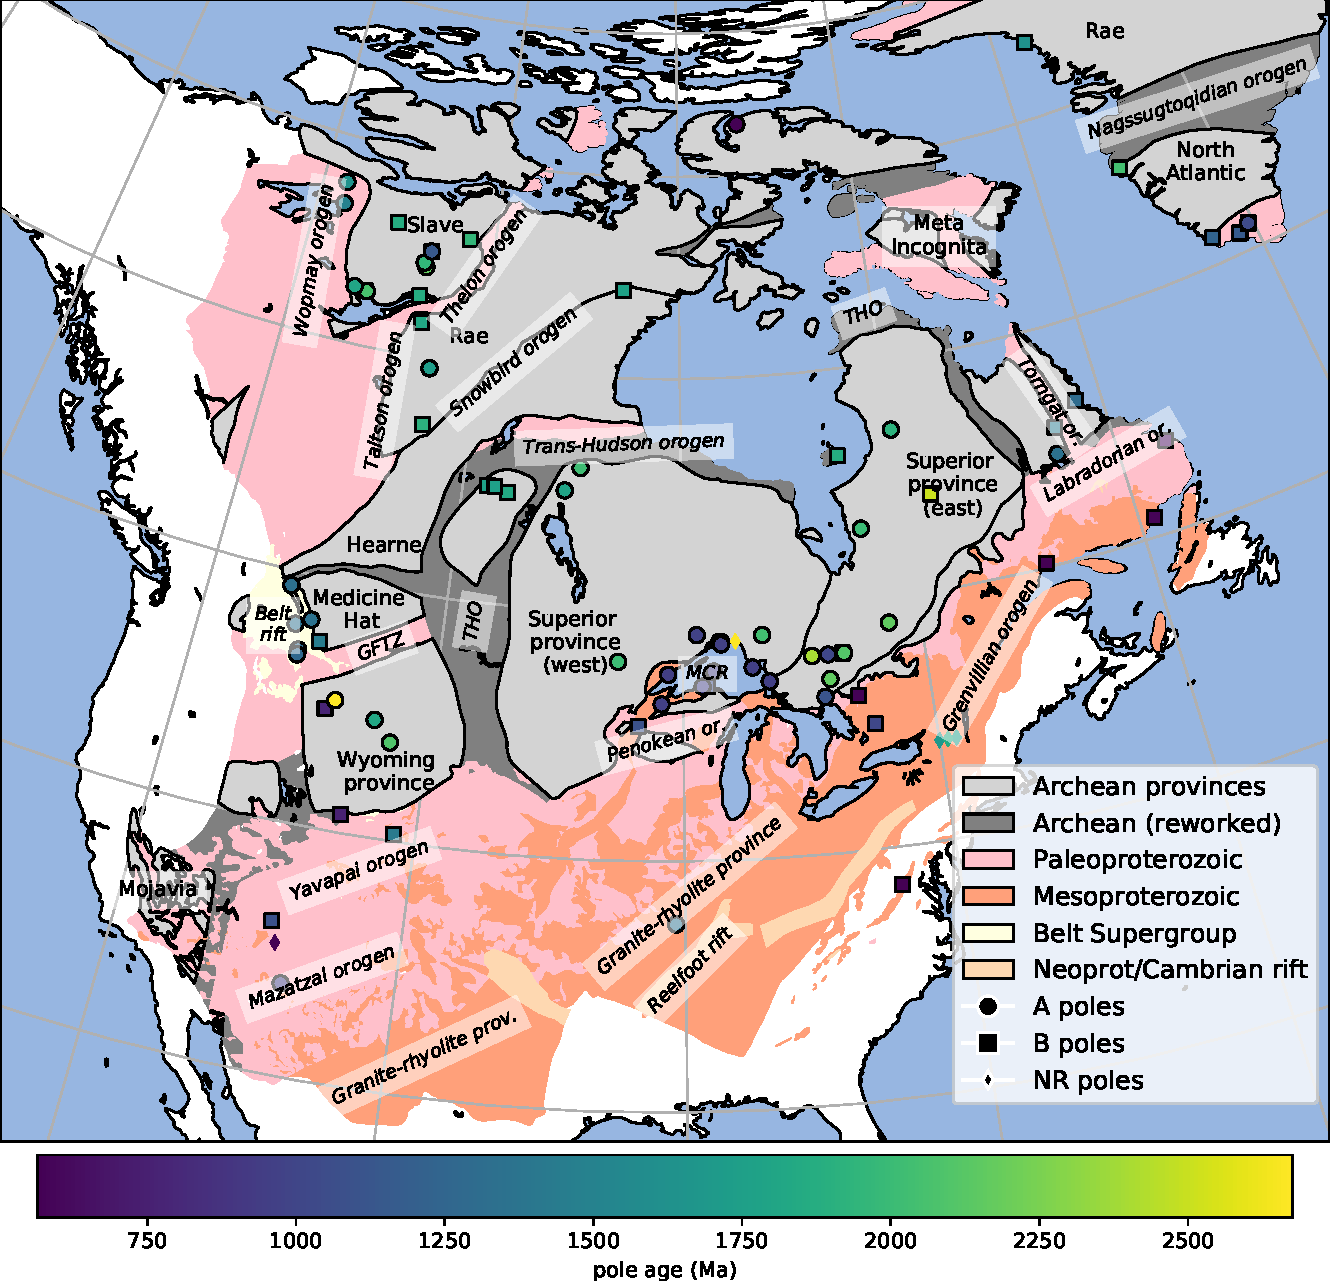
\includegraphics[width=\textwidth]{Figures/Fig1_map.pdf}
\caption{\small{\textbf{Simplified map of Laurentia showing the location of Archean provinces (labeled with text) and younger Paleoproterozoic and Mesoproterozoic crust (simplified from \citealp{Whitmeyer2007a}). The localities from which the compiled Precambrian paleomagnetic poles were developed are shown and colored by age. The circles (A rated poles) and squares (B rated poles) have been assessed by the Nordic workshop panel while the diamonds are additional not-rated results from the Paleomagia database.}}}
\label{fig:Laurentia_map}
\end{figure} 

Crustal growth also progressed at this time in the Paleoproterozoic through accretionary orogenesis. This accretion occurred within the Wopmay orogen through ca. 1.88 Ga arc-continent collision that led to the accretion of the Hottah terrane (the Calderian orogeny) and the subsequent emplacement of the Great Bear magmatic zone from ca. 1.88 to 1.84 Ga \citep{Hildebrand2009a}. Coeval with the Trans-Hudson orogeny was the perphiral Penokean orogeny on the southern margin of the Superior province with the last evidence of that orogeny being ca. 1.78 undeformed plutons of the East Central Minnesota Batholith \citep{Holm2005a}. 

In the paleogeographic model framework of \cite{Pehrsson2015a}, the collisions of provinces and terranes leading up to the Trans-Hudson orogeny mark the initial phase of assembly of the supercontinent Nuna. The Trans-Hudson orogeny itself is taken to be the terminal collision associated with the closure of the Manikewan Ocean that had previous been a large oceanic tract separating the Superior province from the composite Slave+Rae+Hearne+Nain provinces (often referred to as the Churchill domain or plate; e.g. \citealp{Skipton2016a, Weller2017a}). This model posits that this period terminal collision is not only associated with the amalgamation of Laurentia, but is also associated with the assembly of the supercontinent Nuna that is hypothesized to include other major Paleoproterozoic cratons including Siberia, Congo/S\~ao Francisco, West Africa, and Amazonia \citep{Whitmeyer2007a, Pehrsson2015a}. 

Following the Trans-Hudson orogeny, the locus of orogenesis migrated to the exterior of Laurentia. This change marks a shift in the predominant style of Laurentia's growth as subsequent crustal growth occurred dominantly through accretion of juvenile crust along the southern and eastern margin of the nucleus of Archean provinces (\citealp{Whitmeyer2007a}; Figs. \ref{fig:Laurentia_map} and \ref{fig:tectonic_history}). Determining the extent of these belts is complicated by poor exposure of them in the Midcontinent relative to the exposure of the Archean provinces throughout the Canadian shield. Major growth of Laurentia following the amalgamation of these Archean provinces occurred associated with the arc-continent collision of the ca. 1.71 to 1.68 Ga Yavapai orogeny which is interpreted to have resulted from the accretion of a series of arc terranes that collided with each other and Laurentia \citep{Whitmeyer2007a}. Yavapai accretion was followed by widespread emplacement of granitoid intrusions \citep{Whitmeyer2007a}. These intrusions are hypothesized to have stabilized the juvenile accreted terranes that subsequently remained part of Laurentia \citep{Whitmeyer2007a}. Subsequent accretionary orogenesis of the ca. 1.65–1.60 Ga Mazatzal Orogeny and associated plutonism lead to further crustal growth in the latest Paleoproterozoic \citep{Whitmeyer2007a}. Laurentia's growth continued in the Mesoproterozoic along the southeast margin through further juvenile terrane and arc accretion. An interval of major plutonism occurred ca. 1.48–1.35 Ga leading to the formation of A-type granitoids throughout both Mesoproterozoic and Paleoproterozoic provinces. This plutonism is likely due to crustal melting within a back-arc region of ca. 1.50 to 1.43 Ga accretionary orogenesis \citep{Bickford2015a}. Younger magmatic activity ca. 1.37 Ga  of the Southern Granite–Rhyolite Province suggests a similar tectonic setting of accretionary orogenesis at that time \citep{Bickford2015a}. 

\begin{figure}
\centering
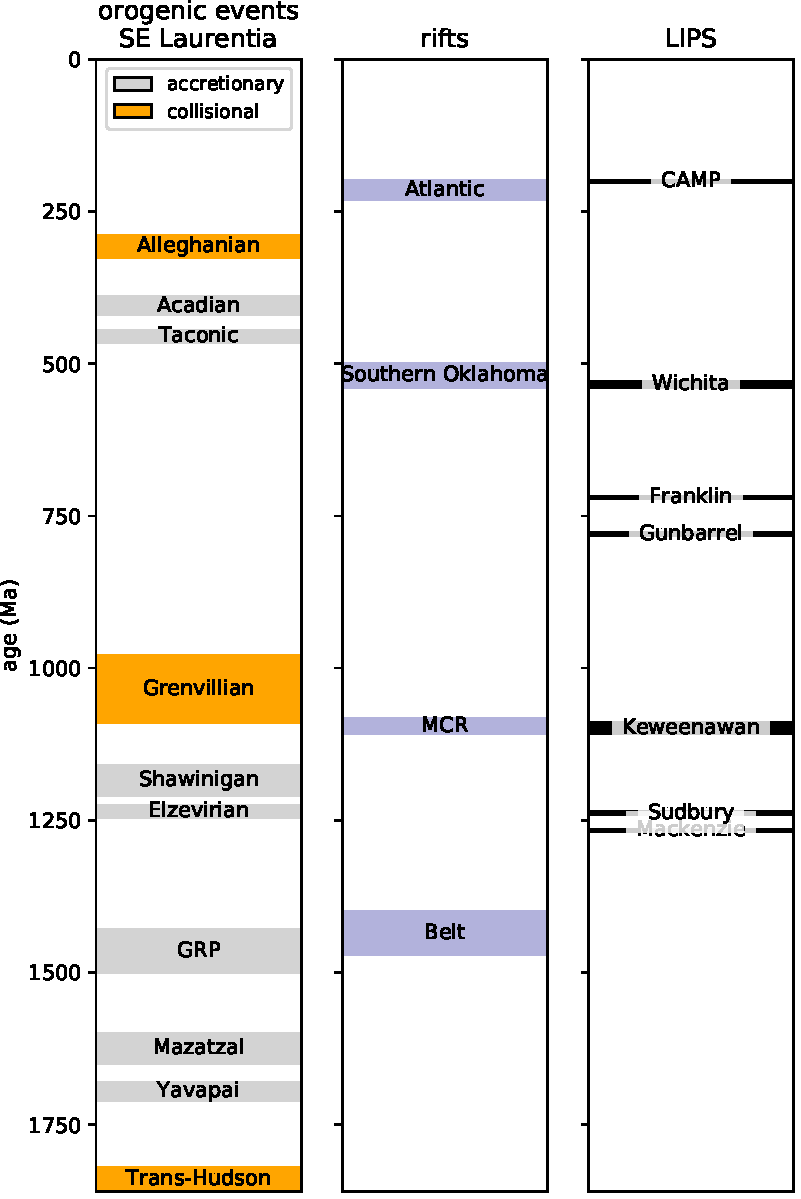
\includegraphics[width=4in]{Figures/Tectonic_history.pdf}
\caption{\small{\textbf{Summary of Laurentia's tectonic history over the past $\sim$1.8 billion years.} Brief summaries and references related to the orogenic and rifting episodes are given in the text. Note that the Penokean orogeny overlaps with the Trans-Hudson orogeny and is not shown.}}}
\label{fig:tectonic_history}
\end{figure}

Accretionary orogenesis continued along the (south)east margin of Laurentia with the arc-continent collision of the ca. 1.25–1.22 Ga Elzevirian orogeny \citep{McLelland2013a}. The subsequent ca. 1.19 to 1.16 Ga Shawinigan orogeny is interpreted to be due to the accretion of a terrane comprised of amalgamated arc volcanics and associated metasediments and is followed by a period of tectonic quiescence on the eastern margin of Laurentia until the collision orogenesis of the Grenvillian orogeny \citep{McLelland2010a}. In the latest Mesoproterozoic (ca. 1.11-1.08 Ga), a major intracontinental rift co-located with a large igneous province formed in Laurentia's interior leading to extension within the Archean Superior province and Paleoproterozoic provinces. This Midcontinent Rift lead to the formation of a thick succession of volcanics and mafic intrusions that are well-preserved in Laurentia's interior.  Midcontinent Rift development ceased as major collisional orogenesis of the Grenvillian orogeny began \citep{Swanson-Hysell2019a}. The Grenvillian orogeny was a protracted interval of continent-continent collision (ca. 1.09 to 0.98 Ga) leading to amphibolite to granulite facies metamorphism through the orogen. The orogeny is interpreted to have resulted in the development of a thick orogenic plateau \citep{Rivers2008a}.

There was significantly less crustal growth on the western margin of Laurentia (Fig. \ref{fig:Laurentia_map}) and the Mesoproterozoic tectonic history is not as well elucidated as on the southern to eastern margin. The 15 to 20 km thick package of sedimentary rocks of the Belt-Purcell Supergroup is associated with ca. 1.47 to 1.40 intracontinental rift -- the tectonic setting of which is debated. \citet{Hoffman1989a} proposed that it may be a remanent back-arc basin trapped within a continent while others envision it as being associated with continental rifting along the margin associated with separation of a conjugate continent \citep[e.g.]{Jones2015a}. This region is interpreted to have been subsequently deformed during a ca. 1.36 to 1.33 event known as the East Kootenay orogeny \citep{McMechan1982a, Nesheim2012a, McFarlane2015a}. 

This late Paleoproterozoic and Mesoproterozoic tectonic history provides significant constraints on paleogeographic reconstructions. In particular, the long-lived history of accretionary orogenesis along the southeast (present-day coordinates) of Laurentia from the initiation of the Yavapai orogeny (ca. 1.71 Ga) to the end of the Shawinigan orogeny (ca. 1.06 Ga) requires a long-lived open margin without a major conjugate continent up until the time of terminal Grenvillian orogeny collision \citep{Karlstrom2001a}. This constraint is incorporated into models such as that of \citet{Pehrsson2015a} which maintain a long-lived convergent margin throughout the Mesoproterozoic, but in some reconstructions other continental blocks are reconstructured into positions that are seemingly incompatible with this record of accretionary orogenesis (e.g. Amazonia in \citealp{Elming2009a}). The high-grade metamorphism associated with the Ottawan phase of the Grenvillian orogeny itself requires a collision between Laurentia and (an)other continent(s) ca. 1080 Ma -- the geological observation of which first lead to the formulation of the hypothesis of the supercontinent Rodinia \citep{Hoffman1991a}. That the Laurentia margin experienced large-scale continent-continent collision at the time of the Ottawan Phase of the Grenvillian orogeny that is recorded in Texas, up through the Blue Ridge Appalachian inliers, through Ontario and up to the Labrador Sea remains a strong piece of evidence that a supercontinent or (proto)supercontinent formed at the 1.0 Ga Mesoproterozoic to Neoproterozoic transition.

The subsequent Neoproterozoic tectonic history of Laurentia is dominantly a record of rifting. Along the western margin of Laurentia, small-scale rifting occurred ca. 780 to 720 Ma leading to deposition in basins that is recorded from the Death Valley region of SW Laurentia up to the Mackenzie Mountains of NW Laurentia \citep{Rooney2017a}. However, this extensional basin development is relatively minor and predates the more significant rifting that lead to passive margin thermal subsidence that did not occur until the Ediacaran (closer to the ca. 539 Ma Neoproterozoic-Phanerozoic boundary; \citealp{Bond1984a, Levy1991a}). The emplacement of the ca. 780 Ma Gunbarrel large igneous province along this margin and the subsequent extension recorded in the basins is commonly interpreted to be associated with the break-up of Laurentia and a conjugate continent to the western margin. If this interpretation is correct, it is unclear why there would be minimal thermal subsidence until the Ediacaran (post 635 Ma as in \citealp{Levy1991a} and \citealp{Witkosky2018a}). The geological evidence therefore supports active tectonism along the western margin of Laurentia, but suggests that more dramatic lithospheric thinning occurred later than the timing of rifting typically implemented in models of Rodinia break-up. One possibility, along the lines of that proposed in \citet{Ross1991a}, is that ca. 780 Ma extensional tectonism is an inboard record of rifting and passive margin development that occurred further outboard. In this model, subsequent continent rifting that drove lithospheric thinning, perhaps associated with the departure of a microcontinent fragment rather than an already departed major conjugate continent, would be the cause of Ediacaran to Cambrian thermal subsidence. The margin that did experience large-scale rifting and associated passive margin thermal subsidence earlier in the Neoproterozoic is the northeast Greenland margin. Available geochronological constraints and thermal subsidence modeling indicate ca. 820 Ma rifting followed by thermal subsidence of a stable platform \citep{Maloof2006a, Halverson2018a}. These data suggest that conjugate continental lithosphere rifted away from northeast Greenland at the time. 

Extensive rifting that was followed by thermal subsidence occurred along the southeast to east Laurentia margin leading up to the Neoproterozoic-Phanerozoic boundary and is interpreted to be associated with the opening of the Iapetus ocean. A record of this rifting is preserved as rift basins that were part of failed arms (Rome trough, Reelfoot rift and Oklahoma aulacogen) as well as prolonged Cambrian to Ordovician passive margin thermal subsidence along the margin \citep{Bond1984a,Whitmeyer2007a}. The age of igneous intrusions that have been interpreted to be rift-related play a significant role in interpretations of this  history such as in the rift development model of \citet{Burton2010a}. In this model, spatially-restricted rifting occurs ca. 760 to 680 Ma in the region of modern-day North Carolina and Virginia. Ca. 620-580 Ma rifting initiates in the region from modern-day New York to Newfoundland and by ca. 580 to 550 Ma rifting extends along the length of Laurentia's eastern margin. The last phases of this rifting are associated with the separation of the Argentine pre-Cordillera Cuyania terrane. Cuyania is widely interpreted be a rifted fragment of SE Laurentia that separated associated with this early Cambrian rifting and subsequently became part of Gondwana when it collided with other terranes in the vicinity of the Rio de Plata craton during the Ordovician Famatinian orogeny \citep{Martin2019a}. As with other rifts, it is difficult to distinguish the separation of a cratonic fragment as a microcontinent from the rifting of a major craton as the record that lingers on the craton is similar. One interpretation is that there was successful break-up along the eastern margin during the ca. 580 to 550 Ma interval of rifting prior to the ca. 539 Oklahoma aulacogen rifting that liberated the Cuyania microcontinent. The Maz–Arequipa–Rio Apa (MARA) block MARA block with which Cuyania collided \citep{Martin2019a} is likely a product of such rifting. Orogenesis between the MARA block and the Rio de Plata and Kalahari in the ca. 530 Ma Pampean orogeny \citep{Casquet2018a} predated the collision of Cuyania during the ca. 460 Famatinian orogeny. 

The eastern margin of Laurentia then went through the cycle of Appalachian orogenesis. As is visualized in Figure \ref{fig:tectonic_history}, there are parallels between the Grenville orogenic interval and the Appalachian one in that there was a period of arc-continent collision (Shawinigan orogeny in the Grenville interval; Taconic orogeny in the Appalachian period) followed by microcontinent accretion (Llano in the Grenville interval; Acadian in the Appalachian interval) that culminated in large-scale continent-continent collision (Grenvillian orogeny in the Grenville interval; Alleghanian in the Appalachian interval). These similarities are the consequence of an active margin facing an ocean basin that was progressively consumed until its consumption resulted in continent-continent collision. In the case of the Grenville interval this terminal collision is interpreted to be associated with the assembly of the supercontinent Rodinia and in the Appalachian interval it is interpreted to be associated to with the assembly of the supercontinent Pangea.

Even without considering other continents on Earth, the geological record of Paleoproterozoic collisional of Archean provinces combined with accretionary orogenesis at that time and through the rest of the Paleoproterozoic and Mesoproterozoic provides very strong evidence for mobile plate tectonics driving Laurentia's evolution throughout the past 2 billion years. This tectonic history inferred from geological data can be enhanced through integration with the paleomagnetic record.

\section*{Paleomagnetic pole compilation}

In this chapter, I will focus on the compilation of paleomagnetic poles developed through the Nordic Paleomagnetism Workshops with some additions and modifications. The Nordic Paleomagnetism Workshops have taken the approach of using expert panels to assess paleomagnetic poles and assign them grades meant to convey the confidence that the community has in these results. While many factors associated with paleomagnetic poles can be assessed quantitatively such as the Fisher statistics and the precision of geochronological constraints, other aspects such as the degree to which available field tests constrain the magnetization to be primary require expert assessment. The categorizations used by the expert panel are `A' and `B' with the last panel meeting occuring in Fall 2017 in Leirubakki, Iceland. An `A' rating refers to poles that are judged to be of such high-quality that they provide essential constraints that should be satisfied in paleogeographic reconstructions. A `B' rating is associated with poles that are judged to likely provide a high-quality constraint, but have some deficiency such as remaining ambiguity in the demonstration of primary remanence or the quality/precision of available geochronologic constraints. Additional poles that were not given an `A' or `B' classification at the Nordic Workshops are referred to as not-rated (`NR'). These additional poles are taken from the Paleomagia database \citep{Veikkolainen2013a}

Prior to the termination of the Trans-Hudson orogeny (before 1.8 Ga), I consider paleomagnetic poles with respect to the individual Archean cratons. There are poles in the compilation for the Slave, Wyoming, Rae, Superior and Nain provinces prior to Laurentia amalgamation. These data provide an opportunity to re-evaluate the paleomagnetic evidence for relative motions between Archean provinces prior to Laurentia assembly. Following the termination of this orogeny (after 1.8 Ga), I consider poles from all the respective provinces and terranes to reflect the position of all of Laurentia. A lingering question raise in \citet{Hoffman198a} that still lingers is whether the Archean provicnes each had independent drit histories with significant speraation ro whether they have shared historieds before experiencing fragmantation and remamalgamation.

For the Superior province, an additional complexity is that paleomagnetic poles from Siderian to Rhyacian Period (2.50 to 2.05 Ga) dike swarms, as well as deflection of dike trends, support an interpretation that there was substantial Paleoproterozoic rotation of the western Superior province relative to the eastern Superior province across the Kapuskasing Structural Zone \citep{Bates1991a, Evans2010a}. This interpretation is consistent with the hypothesis of \citet{Hoffman1988a} that Kapuskasing Structural Zone represents major intracratonic uplift related to the Trans-Hudson orogeny. \cite{Evans2010a} propose an Euler rotation of (51\textdegree N, 85\textdegree W, -14\textdegree CCW) to reconstruct western Superior relative to eastern Superior and interpret that the rotation occured in the time interval of 2.07 to 1.87 Ga.  I follow this interpretation and group the poles into Superior (West) and Superior (East). These poles are shown in Table 1 both in their initial reference frame and rotated into the other Superior reference frame. Uncertainty remains with respect to whether the ca. 1.88 Ga Molson dikes pole pre-dates or post-dates this rotation and thus for the time-being should be considered solely in the western Superior province reference grame. 

Following Laurentia's amalgamation, poles from each part of the Laurentia can be considered to reflect the position of the entire composite craton. It is worth considering the possibility that poles from zones of Paleoproterozoic and Mesoproterozoic accretion could be allochthonous to the craton. \cite{Hall201Xa} argued that this was the case for late Mesoproterozoic and early Neoproterozoic poles from east of the Grenvillian allochothon boundary fault. However, the majority of researchers have considered these poles to post-date major differential motion and be associated with cooling during collapse of thick plateau developed during continent-continent collision (e.g. \cite{}). Poles with a B-rating are also included in the composite that come from Greenland, Svalbard and Scotland. These terranes were once part of contiguous Laurentia, but have subsequently rifted away. These poles need to be rotated into the Laurentia reference frame prior to use for tectonic reconstruction and I apply the following rotations:

\begin{itemize}
\item Laurentia-Greenland.  1202 1800.0   67.5 -118.5  -13.8  1000 !Rotation of Greenland to Laurentia
\item Laurentia-Scotland 1022 1800.0   73.0   96.5  -22.0  1000 !Rotate (proto-)Scotland to Laurentia-Greenland fit according to Darabi2004
\item Laurentia-Svalbard 3301 1275.0  -81.0  125.0   68.0  1000 !Rotate Svalbard to Laurentia in fit that works well with East Greenland basin (Maloof et al., 2006 rotation)
\end{itemize}


To make an argument that differential plate tectonic motion began in the Neoproterozoic is to ignore a vast breadth and depth of geological and paleomagnetic data.

\bibliographystyle{gsabull}
\small\bibliography{../references/allrefs}

\end{document}